\documentclass[border=6pt]{standalone}
\usepackage{tikz}
\usepackage{pgfplots}
\pgfplotsset{compat=1.18}
\usetikzlibrary{arrows.meta,positioning,shapes.geometric,fit,backgrounds,calc,decorations.pathreplacing,patterns}
\usetikzlibrary{pgfplots.groupplots}
\tikzset{
  blk/.style={rectangle, rounded corners=2pt, draw=black!70, thick, fill=blue!6,
              minimum height=8mm, minimum width=20mm, align=center, font=\small},
  io/.style={rectangle, rounded corners=6pt, draw=black!70, thick, fill=green!8,
             minimum height=8mm, align=center, font=\small},
  proc/.style={rectangle, draw=black!70, thick, fill=orange!10, minimum height=8mm,
               align=center, font=\small},
  dec/.style={diamond, aspect=2, draw=black!70, thick, fill=yellow!15, align=center, font=\footnotesize},
  warnbox/.style={rectangle, rounded corners=2pt, draw=red!60!black, thick, fill=red!7,
                  minimum height=8mm, align=center, font=\small},
  oklbox/.style={rectangle, rounded corners=2pt, draw=green!45!black, thick, fill=green!8,
                 minimum height=8mm, align=center, font=\small},
  ar/.style={-{Latex[length=2mm]}, thick},
  arl/.style={-{Latex[length=2mm]}, thick, dashed, draw=black!55},
  lbl/.style={font=\footnotesize\itshape, text=black!60},
}
\definecolor{good}{RGB}{34,139,34}
\definecolor{bad}{RGB}{178,34,34}
\definecolor{warn}{RGB}{218,165,32}
\definecolor{pesblue}{RGB}{0,45,98}
\definecolor{complete}{RGB}{30,125,79}
\definecolor{partial}{RGB}{176,106,0}
\definecolor{blocked}{RGB}{166,43,43}
% --- figure-local styles -------------------------------------------------
\tikzset{
  stage/.style={rectangle, rounded corners=2pt, draw=black!65, thick, fill=blue!6,
                font=\scriptsize, align=center, inner sep=3.5pt, minimum height=7.5mm},
  pill/.style={rectangle, rounded corners=2pt, draw=black!40, fill=white,
               font=\tiny, align=center, inner sep=2.0pt, minimum height=5.0mm},
  pilld/.style={rectangle, rounded corners=2pt, draw=complete!70!black, thick,
                fill=complete!9, font=\tiny, align=center, inner sep=2.0pt,
                minimum height=5.0mm},
  rrowlab/.style={font=\tiny\bfseries, text=black!65, anchor=west, align=left},
  sink/.style={rectangle, rounded corners=2pt, draw=black!55, thick, fill=black!6,
               font=\tiny, align=left, inner sep=3.5pt, text width=3.0cm},
  consumer/.style={rectangle, rounded corners=2pt, draw=black!50, thick, fill=orange!7,
                   font=\tiny, align=left, inner sep=4pt, text width=4.05cm},
}
\begin{document}
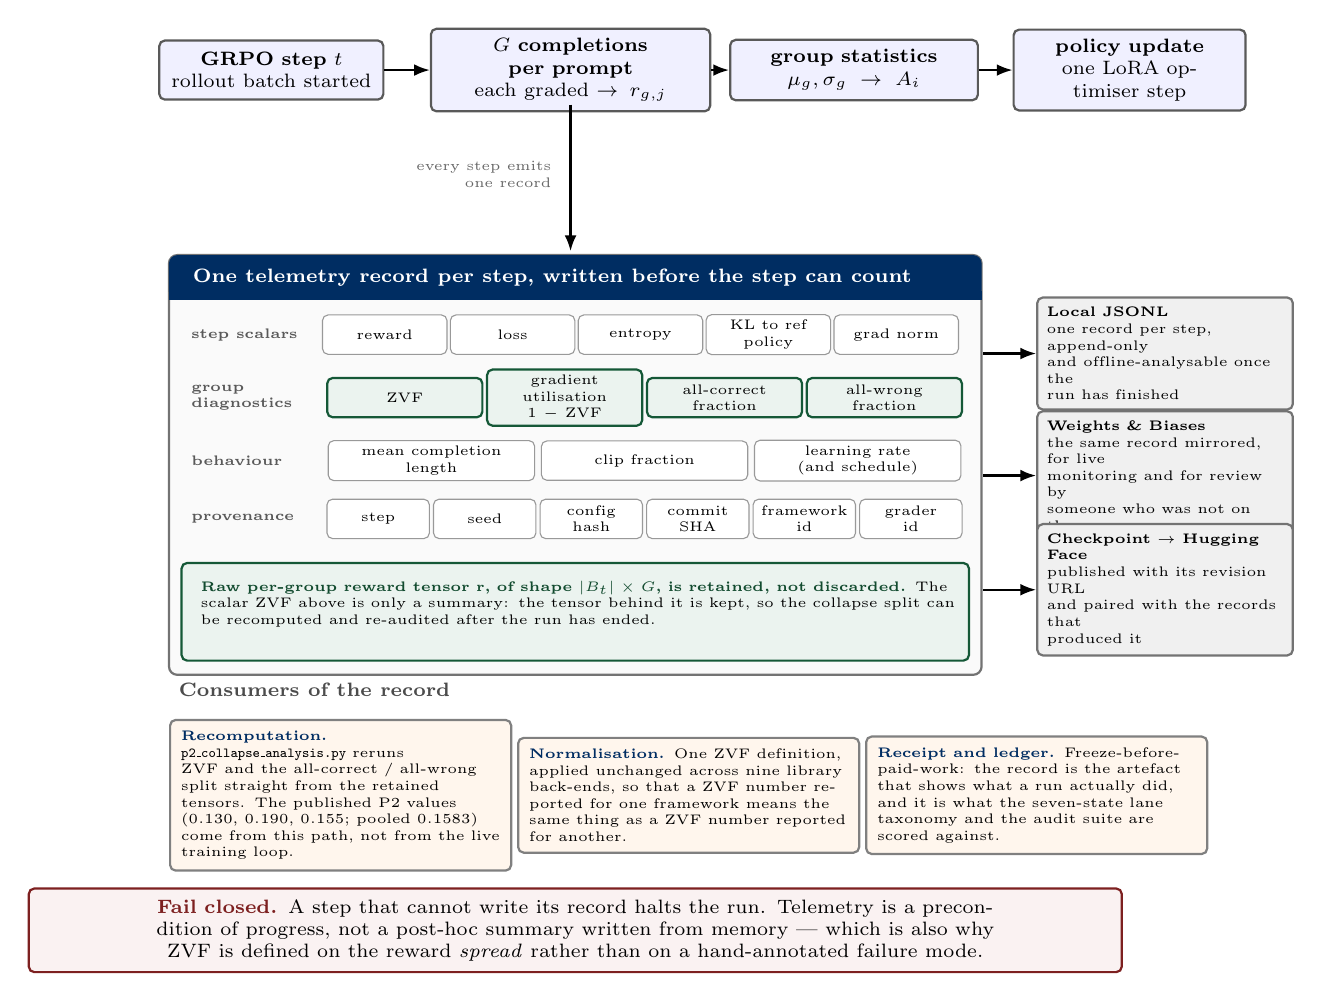
\begin{tikzpicture}

% ===================== 1. what one step produces =========================
\node[stage, text width=2.6cm] (s1) at (-5.3,0) {\textbf{GRPO step $t$}\\rollout batch started};
\node[stage, text width=3.3cm] (s2) at (-1.5,0) {\textbf{$G$ completions per prompt}\\each graded $\rightarrow r_{g,j}$};
\node[stage, text width=2.9cm] (s3) at (2.1,0) {\textbf{group statistics}\\$\mu_g,\sigma_g \rightarrow A_i$};
\node[stage, text width=2.7cm] (s4) at (5.6,0) {\textbf{policy update}\\one LoRA optimiser step};
\draw[ar] (s1) -- (s2);
\draw[ar] (s2) -- (s3);
\draw[ar] (s3) -- (s4);

% ===================== 2. the record itself ==============================
\fill[black!2, rounded corners=3pt] (-6.60,-2.35) rectangle (3.72,-7.68);
\draw[black!55, thick, rounded corners=3pt] (-6.60,-2.35) rectangle (3.72,-7.68);
\fill[pesblue, rounded corners=3pt] (-6.60,-2.35) rectangle (3.72,-2.92);
\fill[pesblue] (-6.60,-2.80) rectangle (3.72,-2.92);
\node[white, font=\scriptsize\bfseries, anchor=west] at (-6.42,-2.635)
  {One telemetry record per step, written before the step can count};

\draw[ar] (-1.5,-0.44) -- (-1.5,-2.30);
\node[font=\tiny, text=black!60, anchor=east, align=right] at (-1.62,-1.32)
  {every step emits\\one record};

% ---- field rows (pitch: 5 / 4 / 3 / 6 pills) ----------------------------
\node[rrowlab] at (-6.44,-3.36) {step scalars};
\foreach \j/\t in {0/{reward},1/{loss},2/{entropy},3/{KL to ref\\policy},4/{grad norm}}
  \node[pill, text width=1.44cm] at (-3.86+1.624*\j,-3.36) {\t};

\node[rrowlab] at (-6.44,-4.16) {group\\diagnostics};
\foreach \j/\t in {0/{ZVF},1/{gradient\\utilisation $1-\mathrm{ZVF}$},2/{all-correct\\fraction},3/{all-wrong\\fraction}}
  \node[pilld, text width=1.83cm] at (-3.605+2.03*\j,-4.16) {\t};

\node[rrowlab] at (-6.44,-4.96) {behaviour};
\foreach \j/\t in {0/{mean completion\\length},1/{clip fraction},2/{learning rate\\(and schedule)}}
  \node[pill, text width=2.48cm] at (-3.267+2.707*\j,-4.96) {\t};

\node[rrowlab] at (-6.44,-5.70) {provenance};
\foreach \j/\t in {0/{step},1/{seed},2/{config\\hash},3/{commit\\SHA},4/{framework\\id},5/{grader\\id}}
  \node[pill, text width=1.16cm] at (-3.943+1.353*\j,-5.70) {\t};

% ---- the retained tensor sub-box ---------------------------------------
\draw[complete!70!black, thick, rounded corners=2pt, fill=complete!9]
  (-6.44,-6.26) rectangle (3.56,-7.50);
\node[font=\tiny, align=left, anchor=north west, text width=9.7cm] at (-6.32,-6.36)
  {\textbf{\textcolor{complete!60!black}{Raw per-group reward tensor
   $\mathbf{r}$, of shape $|B_t|\times G$, is retained, not discarded.}}
   The scalar ZVF above is only a summary: the tensor behind it is kept, so the
   collapse split can be recomputed and re-audited after the run has ended.};

% ===================== 3. where the record goes ==========================
\node[sink] (k1) at (6.05,-3.60)
  {\textbf{Local JSONL}\\one record per step, append-only\\and offline-analysable once the\\run has finished};
\node[sink] (k2) at (6.05,-5.15)
  {\textbf{Weights \& Biases}\\the same record mirrored, for live\\monitoring and for review by\\someone who was not on the run};
\node[sink] (k3) at (6.05,-6.60)
  {\textbf{Checkpoint $\rightarrow$ Hugging Face}\\published with its revision URL\\and paired with the records that\\produced it};
\draw[ar] (3.74,-3.60) -- (k1.west);
\draw[ar] (3.74,-5.15) -- (k2.west);
\draw[ar] (3.74,-6.60) -- (k3.west);

% ===================== 4. who reads it ==================================
% anchored by its own south edge, well clear of c1.north (which sits at about
% y=-8.31 for this box's text): an anchor=west label here is crossed by the border
\node[font=\scriptsize\bfseries, text=black!70, anchor=south west] at (-6.60,-8.08)
  {Consumers of the record};

\node[consumer] (c1) at (-4.42,-9.21)
  {\textbf{\textcolor{pesblue}{Recomputation.}} \texttt{p2\_collapse\_analysis.py} reruns ZVF and the
   all-correct / all-wrong split straight from the retained tensors. The published P2
   values ($0.130$, $0.190$, $0.155$; pooled $0.1583$) come from this path, not from
   the live training loop.};
\node[consumer] (c2) at (0.00,-9.21)
  {\textbf{\textcolor{pesblue}{Normalisation.}} One ZVF definition, applied unchanged
   across nine library back-ends, so that a ZVF number reported for one framework means
   the same thing as a ZVF number reported for another.};
\node[consumer] (c3) at (4.42,-9.21)
  {\textbf{\textcolor{pesblue}{Receipt and ledger.}} Freeze-before-paid-work: the record is
   the artefact that shows what a run actually did, and it is what the seven-state lane
   taxonomy and the audit suite are scored against.};

\node[rectangle, rounded corners=2pt, draw=blocked!75!black, thick, fill=blocked!6,
      font=\scriptsize, align=center, inner sep=4pt, text width=13.6cm, anchor=north]
  at (-1.44,-10.38)
  {\textbf{\textcolor{blocked!75!black}{Fail closed.}} A step that cannot write its record
   halts the run. Telemetry is a precondition of progress, not a post-hoc summary written
   from memory --- which is also why ZVF is defined on the reward \emph{spread} rather than on
   a hand-annotated failure mode.};

\end{tikzpicture}
\end{document}
